\documentclass{standalone}
\usepackage{tikz}
\usetikzlibrary{bbox, angles, quotes, intersections}
\usetikzlibrary{calc}
\usetikzlibrary{arrows.meta,decorations.pathmorphing,backgrounds,positioning,fit,petri}

%\def\b{0.05}
\def\b{5}
\def\c{\b -1}
\def\rrr{4}
\def\centerarc[#1](#2)(#3:#4:#5)% Syntax: [draw options] (center) (initial angle:final angle:radius)
    { \draw[#1] ($(#2)+({(#5)*cos(#3)},{(#5)*sin(#3)})$) arc (#3:#4:#5); }

\def\beamline[#1](#2)(#3:#4)% Syntax: [draw options] (radius) (initial angle:final angle:radius)
    {  \draw[#1] ({(#2-2*\b)*cos(#4)},-#3/2 * sin(#4)) -- ({(#2-2*\b)*cos(#4)},#3/2 * sin(#4)); 
    \draw ({(1-2*0.05)*cos(90)},{-1/2 * sin(90)}) -- ({(1-2*0.05)*cos(90)},{1/2 * sin(90)});
    }


\begin{document}

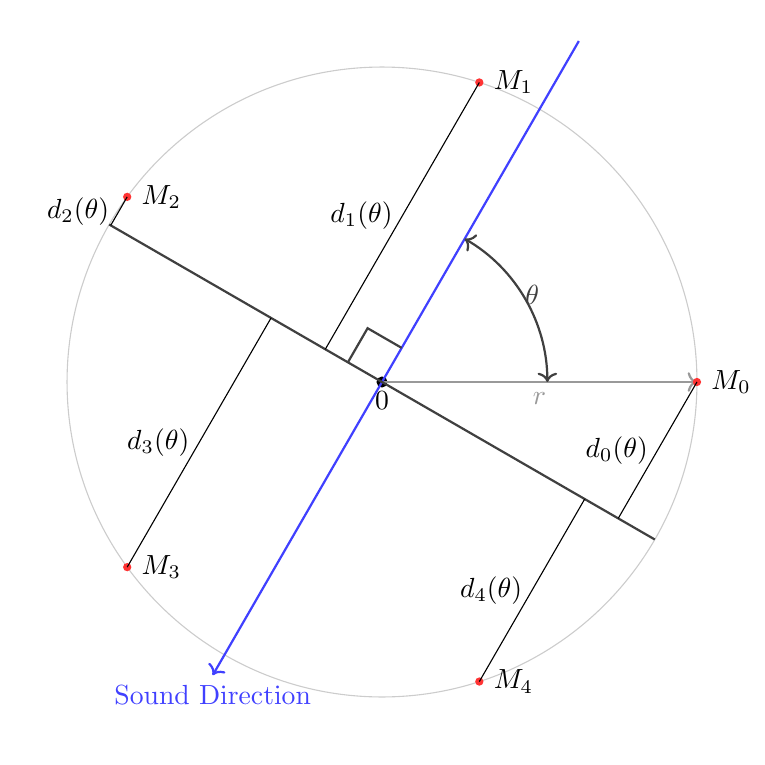
\begin{tikzpicture}
    [
        mymic/.style={circle,fill=red!80, inner sep=0pt,minimum size=3pt},
        wave/.style={white!80!black,thin},
        wave1/.style={white!25!black,thick},
        wave11/.style={white!25!blue,thick},
        angle1/.style={white!25!blue,thick},
        wave2/.style={white!60!black,thick}
    ]
%    \draw[style=help lines,step=0.5cm] (-4,-4) grid (4,4);
    \coordinate[label=below:0] (origin) at (0,0);
    \fill[black] (origin) circle (2pt);
    \draw[wave](origin) circle (\rrr);
   
    \coordinate[] (r0) at (\rrr, 0);
    \coordinate[] (w1) at (60:5);
    \coordinate[] (w2) at (240:\rrr + 0.3);
    \coordinate[] (w3) at (150:\rrr);
    \coordinate[] (w4) at (330:\rrr);

    \draw [->, wave2] (origin) -- (r0) node[midway,below]{$r$};
    \draw [<-, wave11] (w2) node[below]{Sound Direction}  -- (w1) ;
    \draw[wave1, name path=mLine] (w3) -- (w4) ;

    \foreach \i in {0,...,4}
    {
        \node[mymic, label=right:{$M_\i$}] at (\i * 360/\b:\rrr) {};
        \path[name path=line] (\i * 360/\b:\rrr) -- (300 - \i * 360/\b:\rrr);  
            
        \draw[black,name intersections={of=line and mLine,by={Int1}}] (\i * 360/\b:\rrr) -- (Int1)
            node[midway,left]{$d_\i(\theta)$};
%        \fill[red] (\i * 360/8:3) circle (2pt);  
    }

    
    \begin{scope}[transform canvas={rotate=30}]
%        \draw[wave1] (2.898,0) -- (2.898,1);
        
    \end{scope}
    \pic [draw,wave1,angle eccentricity=10,pic text=.]
        {right angle = w3--origin--w1};
    \pic [draw, <->, wave1,
    angle radius=21mm, angle eccentricity=1.05,"$\theta$"] {angle = r0--origin--w1};
    \pgfresetboundingbox
%    \useasboundingbox(-2.6,-2.6)rectangle(2.6,3.6);
    \useasboundingbox(-4.5,-4.5)rectangle(4.5,4.5);
\end{tikzpicture}
\end{document}